\subsubsection{Generative Deep Learning Architectures}

Generative \ac{DL} architectures are a subset of \ac{DL} networks designed to generate new and diverse data samples from a learned distribution.

By finding latent data structures and learning to reproduce the hidden statistics behind observed data, they do so. To achieve this, the model tries to estimate an underlying probability distribution $p_{data}$ when given a set of samples from this distribution. Thus, training a generative model involves selecting the best parameters that reduce some concept of distance/loss/error between the model and the actual distribution. As Huzaifah \cite{huzaifah_deep_2021} states: ``given training data points $X$ as samples from an empirical distribution $p_{data}(X)$, we want to learn a model $p_\theta(X)$, belonging to a model family $M$ that closely matches $p_{data}(X)$, by repeatedly changing model parameters $\theta$''. This is expressed as the problem in equation \ref{eq:generative-models-base}.

\begin{equation} \label{eq:generative-models-base}
    \min_{\theta \in M} d (p_{data}, p_\theta)
\end{equation}

Standard functions for $d$ are displayed in section \ref{sec:loss-functions}.

These models have been applied to various tasks, such as image synthesis, text generation, and audio synthesis. Generative \ac{DL} models have gained popularity recently due to their ability to produce high-quality data and model complex distributions.

This section will present the most used architectures.

\paragraph{Deep Autoregressive Network (DARN)} \label{sec:darn}

First introduced in 2013, \acf{DARN} is an architecture for generative models that are used to generate data by using an \acf{AR} approach \cite{gregor_deep_2014}.

\Ac{AR} models generate data by predicting the following sample in a sequence based on the previous samples. In the case of \acp{DARN}, the model has multiple hidden layers to do so. The idea behind it is to model the data's complex, high-dimensional probability distribution by breaking it down into a series of simple, conditionally independent distributions. This is done by learning a deep neural network that maps inputs to outputs through a series of hidden layers. This allows the network to build up a complex representation of the data distribution over time, capturing complex patterns in the data and ultimately making more precise predictions.

By applying the chain rule of probability, \ac{AR} models can create a feasible density model that breaks down the probability distribution over $n$ time steps \cite{huzaifah_deep_2021}, as shown in equation

\begin{equation} \label{eq:chain-rule}
    p(X) = \prod_{i=1}^n p(x_i|x_1, ..., x_{i-1})
\end{equation}

This method implies that data has a standard sequential order—the present term in the sequence $(x_i)$ depends only on a recent window of preceding terms. Future terms are not taken into account. This is, ultimately, they assume that a data point only depends on previous ones and learn to predict the following sample is given only what has come just prior. The rationale behind this technique is similar to the one that \acp{RNN} employ. In fact, an \ac{RNN} can be seen as an \ac{AR} model that reduces the previous terms to a hidden state rather than giving them directly as input to a layer \cite{huzaifah_deep_2021}. Besides, \ac{AR} models are more straightforward and faster to train. Indeed, an \ac{AR} model is a feedforward model (see Section \ref{sec:feedforward} )which predicts future values from past values. One can imagine a model similar to a feedforward neural network that is not fully connected but with only some connections regarding past inputs. This can be seen in Figure \ref{fig:darn}.

\begin{figure}[ht]
    \centering
    \ctikzfig{figures/2-sota/darn}
    \caption[Deep autoregressive network]{\textbf{\Acf{DARN}} --- The input of each neuron in a given layer is conditioned by the output of the 2 previous neurons in the previous output.}
    \label{fig:darn}
\end{figure}
\paragraph{Variational Autoencoder (VAE)} \label{sec:vae}

Kingma and Welling proposed the concept of \acfp{VAE} in 2013 \cite{kingma_auto-encoding_2022}. The authors proposed a new approach to traditional \acp{AE} that utilizes a variational inference method to model complex distributions in high-dimensional spaces. Thus allowing for the generation of new, unseen data similar to the initial training.

In the realm of \acp{AE}, traditional approaches, as discussed in Section \ref{sec:autoencoders}, aim to map the identity function through the utilization of encoder and decoder networks. The encoder takes the input and transforms it into a compressed vector representation, while the decoder reconstructs the input from this compressed representation. However, Variational Autoencoders (\acp{VAE}) introduce a distinct variation in their approach. Instead of modeling the input as a deterministic vector, the encoder in \acp{VAE} characterizes the input data as a probability distribution across potential representations. This distribution is typically represented by two sets of latent values: one corresponding to the mean and the other to the variance. These latent sets are often modeled using fully connected layers within the architecture.

Consequently, the \ac{VAE} framework imposes a constraint on the embedded vector by confining it to a specified number of points in a hyperplane. Interestingly, this enables us to discard the encoder entirely. By working with a continuous latent space, the decoder of the \ac{VAE} can generate novel and diverse samples akin to the training data. Figure \ref{fig:vae} provides a visual depiction of this concept, illustrating how the decoder operates based on samples from the latent distribution to generate new output.

\begin{figure}[ht]
    \centering
    \ctikzfig{figures/2-sota/vae}
    \caption[Variational autoencoder]{\textbf{\Acf{VAE}} --- The \ac{VAE} encoder operates in a manner comparable to the traditional \ac{AE}, but with a notable distinction. Instead of directly mapping the input to a single latent representation, the \ac{VAE} encoder translates the input into two sets of latent features: the normals and the variances. These latent features are represented in the Figure by the two sets of nodes within the bottleneck of the encoder architecture.}
    \label{fig:vae}
\end{figure}

This was encouraging, as distributions near each other would produce similar outputs. This means, it created smooth changes between data points. The explanation for this is that \acp{VAE} discover low-dimensional parameterized representations of the data \cite{huzaifah_deep_2021}.

For training, these networks use an objective function that aims to minimize the loss between input and output and ensure that the learned distribution is similar to a prior distribution, such as a Gaussian.

However, sometimes during training, the \ac{VAE} can learn to ignore the latent variable and instead rely solely on the decoder network to generate the output. This means that the encoder network outputs the same distribution over the latent space for all input data points, resulting in a collapsed posterior distribution. In other words, the encoder fails to capture the variability in the input data, and the decoder generates outputs that are not diverse.

This phenomenon is known as \textit{posterior collapse}, and it can occur due to various reasons, such as a high reconstruction loss weight or a small latent space size. Posterior collapse can severely impact the performance of the \ac{VAE} and result in poor-quality generated samples.

These models can be used for any generative task, such as computer vision, natural language processing, and sound generation.

\paragraph{Generative Adversarial Network (GAN)} \label{sec:gan}

The paper ``Generative Adversarial Networks'' by Goodfellow et al. \cite{goodfellow_generative_2014} introduced a novel framework for generative modeling using deep neural networks. The main idea behind \acp{GAN} is to train two neural networks simultaneously, one generator and one discriminator.

By transforming a random noise vector $z$ into a target distribution in some data space $\hat{X}$ (for example, spectrograms), the generator network $G$ produces new samples. Meanwhile, the discriminator $D$ attempts to tell apart synthetic and real data; that is, $D$ assigns the input data, whether it is $X$ or $\hat{X}$, a categorical label based on whether it believes the input originated from the actual data distribution $p(X)$ or the model distribution $p(z)$. Figure \ref{fig:gan} shows this process.


\begin{figure}[ht]
    \centering
    \ctikzfig{figures/2-sota/gan}
    \caption[Generative adversarial network]{\textbf{\Acf{GAN}} --- A random noise vector $\vec{z}$ is passed through the generator in $G(\vec{z})$ to create the synthetic sample $\hat{X}$. Both this and the real sample $X$ are passed to the discriminator $D$ that predicts which of the samples is the real one. It is important to notice that in this illustration, the circles represent entire neural networks and not simply neurons.}
    \label{fig:gan}
\end{figure}

Using a minimax optimization framework, the networks are trained in an adversarial way. The goal is that $G$ generates a fake sample $\hat{X}$ that is given to $D$ along with a real one $X$. This network then has to identify which is genuine and which is fabricated. $D$ is trained to increase the probability of telling apart the real from the fake data. While $G$ is trained at the same time for the opposite objective, that is, to deceive $D$ by minimizing $\log(1 - D(G(z)))$ \cite{huzaifah_deep_2021}. $G$ and $D$ are trained in turns until a Nash equilibrium is achieved.

When $G$ creates flawless fake data that cannot be told apart from real data, a Nash equilibrium is reached. $D$ has no clue whether the data is real or fake and just makes random guesses about the input label. In this situation, $G$ performs at its best, and $D$ performs at its worst. The models cannot get any better than this. This is a perfect scenario that requires effort to attain in reality. It is worth noting that the generator never sees the training samples, only the feedback given by the discriminator \cite{huzaifah_deep_2021}.

Once the training is done, the discriminator is thrown away, and the generator can be used to draw samples from the learned distribution of the real data. The generator has learned to associate random vectors with data samples in the target domain. These vectors usually represent some features. As a result, they cluster output data with similar features to nearby input values, offering a natural way of exploring output data with different attributes. This implies that similar input vectors will produce similar outputs \cite{huzaifah_deep_2021}.

Although this technique has seen great success in producing high-resolution images, it still needs to improve in the audio domain as the sections in Section~\ref{sec:related-work} show. Besides that, even in ideal settings, it has some drawbacks. For instance, the fact that the training of the whole model implies the training of two different networks makes it unstable. It is easy to get stuck at a sub-optimal nash equilibrium. One such example is mode collapse, where the generator produces limited variations of the target distribution.

\Acfp{DARN} (see Section \ref{sec:darn}) represented the state-of-the-art in neural audio synthesis for a long time. These models are good at learning local latent structure, this is, the features of sounds over brief periods. However, they struggle with longer-term features. Besides, \acp{DARN} are very slow because they generate waveforms one sample at a time. \Acp{GAN} are capable of modeling global latent structure since they build the output as a whole; moreover, after training, they generate way faster \cite{tahiroglu_-terity_2020}, showing promising features for audio generation.
\paragraph{Normalizing Flow Models} \label{sec:flow-model}

Normalizing flow models provide a flexible and robust framework for generative modeling and were first introduced in 2015 \cite{rezende_variational_2016}.

The main idea is to use the change of variables in the probability distributions technique to convert simple distributions into more complicated ones. This technique requires applying a transformation to a distribution that changes it into another, more intricate, distribution. The entire idea begins with a simple distribution (for instance, Gaussian) for a set of hidden variables $z$. The goal is to change this distribution into a complex one that corresponds to an output $X$. A single transformation is provided by a smooth and reversible function $f$ that can relate $z$ and $X$, such that $X = f (z)$ and $z = f^{- 1}(X)$. Considering the complexity of $X$, one of these transformations might not produce a sufficiently complex distribution. Hence, multiple reversible transformations are combined sequentially, forming a ``flow''. Neural network layers determine each mapping function in the flow \cite{huzaifah_deep_2021}. Figure \ref{fig:normalizing-flows} illustrates this process.

\begin{figure}[ht]
    \centering
    \ctikzfig{figures/2-sota/normalizing-flows}
    \caption[Normalizing flows network]{\textbf{Normalizing flows network} --- This illustration was based on \cite{weng_flow-based_2018} and shows the application of multiple invertible functions $f_k$ composed one after the other in order to build the complex output $z_K = x$ from a simple Gaussian distribution.}
    \label{fig:normalizing-flows}
\end{figure}

Accurately, let $z_0$ be a multivariate random variable with a distribution $p_0(z_0)$ where $p_0$ is, for example, a Gaussian distribution. Then, for $i = 1, ..., K$ where $K$ is the number of flow operations, let $z_i = f_i(z_{i - 1})$ be a sequence of random multivariate variables. $f_i^{-1}$ should exist for training to occur. The final output $z_K$ models the target distribution.

Normalizing flow models are flexible, meaning they can model various distributions by stacking multiple normalizing flows to form a deep network. This allows it to capture complex relationships between variables in the data.

These models have been proven effective for the generative modeling of high-dimensional data.

In the generative scene, these models are distinguished from the previously mentioned ones because they can speed up the generations and modeling processes \cite{huzaifah_deep_2021}.
\paragraph{Diffusion Models} \label{sec:diffusion}

Until the proliferation of diffusion models, the architecture most used for data generation was the \ac{GAN} (Section \ref{sec:gan}). The problem is that \acp{GAN} are hard to train. For instance, mode collapse can happen. In mode collapse, the generator always generates the same data that fools the discriminator.

\textit{Diffusion models} \cite{sohl-dickstein_deep_2015} simplify this generation process into more intuitive small steps where the work of the network is lighter and is run multiple times. This is done by taking inspiration from non-equilibrium thermodynamics. These models define a Markov chain of diffusion steps to slowly add random noise to data and then learn to reverse the diffusion process to construct desired data samples from the noise.

Practically, diffusion models use a Markov chain to gradually convert one distribution into another. This chain starts from a simple known distribution (\textit{e.g.} a Gaussian) into a target distribution using a diffusion process. Learning in this framework involves estimating small perturbations to a diffusion process, using a network such as the U-Net (Section \ref{sec:u-net}). Estimating small perturbations is more tractable than explicitly describing the whole distribution with a single, non-analytically-normalizable potential function. This process can be seen in Figure \ref{fig:diffusion}

\begin{figure}[ht]
    \centering
    \ctikzfig{figures/2-sota/diffusion}
    \caption[Diffusion model]{\textbf{Diffusion model} --- This illustration was based on \cite{ho_denoising_2020} and shows the process of applying Gaussian noise to an image sample through multiple steps $q(X_t|X_{t-1})$. The model will then learn the operation $p$ that transforms $X_t$ into $X_{t-1}$ with $p(X_{t-1}|X_t)$ and so on until $X_0$. At this point, the model has generated a new data sample.}
    \label{fig:diffusion}
\end{figure}

The ultimate goal is to define a forward (or inference) diffusion process which converts any complex data distribution into a simple, tractable distribution and then learn a finite-time reversal of this diffusion process which defines the generative model distribution \cite{sohl-dickstein_deep_2015}.

One problem is that one needs to decide how much noise one wants to increment per iteration. For instance, if one decides to train a network that directly learns to denoise full Gaussian to a real image, then one is simply training a \ac{GAN} generator. It is easier to remove a small amount of noise per iteration. The amount of noise added per iteration is a hyperparameter called a scheduler. For instance, one can add the same amount of noise per iteration, called the \textit{linear schedule}. Multiple schedules may have different impacts.

For instance, given a linear scheduler, one can define that for $t = x$, the sample would be the original one with $k = x \times 10$ random data points with Gaussian noise. This allows data generation in different timestamps without running through all timestamps. For instance, generating a data sample with $t = 5$ would be as easy as noising $k = 50$ random data points.

To train these networks, one would give pairs of the original data sample $X$ plus a data sample at a random timestamp $X_t$ plus the random step $t$, $X_t = X + N(t)$ where $N$ is a noising function. The network would learn to get the noise from the data given a timestamp. This means that the network would learn to predict $N(t)$ using image segmentation. This will not always be perfect, so the network learns to predict $\tilde{N(t)}$. Then, theoretically, by applying $X_t - \tilde{N(t)}$, one gets $\tilde{X}$, which should be as close as possible to $X$. This process for $t = 50$ is challenging, as most of the data is Gaussian noise. However, applying the process for, for instance, $t = 1$, should be quite easy.

For inference, one gets noisy data $X_t$ and a given timestamp $t$. Applying the network returns $\tilde{N(t)}$ as explained previously. By doing $\tilde{X} = X_t - \tilde{N(t)}$, one generates a bad data sample. But then, the algorithm takes $\tilde{X}$ and applies $N(t - 1)$. This results in another noisy data sample with less noise. This process loops until $t = 0$. By then, a new data sample is generated.
\paragraph{Transformers} \label{sec:transformers}

In 2017, the introduction of the ``Attention is All You Need''~\cite{vaswani_attention_2017} paper marked a significant milestone in \ac{DL}. Although initially introduced for \ac{NLP}, the transformer architecture has proven helpful in various data generation tasks, including audio synthesis as shown in Section~\ref{sec:related-work}. This marked a paradigm shift from the conventional \ac{RNN}-based models, which were earlier widely used, with some incorporating a rudimentary form of the attention mechanism.

In transformers, attention is a key component that allows the model to focus on relevant parts of the input sequence when making predictions. Mathematically, attention can be defined as a weighted sum of values based on their importance or relevance.

Let's break down the mathematical formulation of attention in transformers:

Query \(Q\), Key \(K\), and Value \(V\): These are three linear transformations applied to the input sequence. The query represents the element for which we want to compute attention weights, while keys and values represent all elements in the sequence.

To calculate how much each value contributes to the output for a given query, we compute dot products between the query and all keys:

\begin{equation}
    \text{{scores}} = Q \cdot K^T
\end{equation}

Here, \(\cdot\) represents matrix multiplication, \(K^T\) denotes transpose of matrix \(K\).

The next step is to normalize these scores using a softmax function along dimension 1 (rows) to obtain attention weights that sum up to 1:

\begin{equation}
    \text{{weights}} = \text{{softmax}}(\text{{scores}})
\end{equation}

Finally, we take a weighted sum of values using these normalized attention weights:

\begin{equation}
\begin{split}
    &\text{{attended\_values}} = V \cdot {\text{{weights}}} \\
    &\text{{output}} = {\sum{( {\text{attended\_values} } })}
\end{split}
\end{equation}

Here, $\text{softmax}$ computes exponentiated values scaled by their row-wise sums, while $\text{sum}$ performs summation across rows.

The resulting output represents an attended representation obtained by giving higher weightage/importance to more relevant parts of the input sequence based on similarity with respect to the query. This mathematical formulation allows transformer models to capture long-range dependencies effectively by attending to the pertinent information in the source sequence when generating predictions.

The attention mechanism allows the model to give different importance to different input parts. For instance, let us imagine a translation task English-Portuguese. If naively translated, the sentence ``She is a doctor'' could be translated to ``Ela é um doutor''. However, if, when generating the last word, the model gives some importance to the word ``she'', it might guess that the correct word is ``doutora''.

The key idea behind transformers is to completely disregard the recurrent architecture and only use attention by using self-attention. Self-attention is a mechanism that allows the calculation of the importance of each input element concerning all other elements in the input sequence. This allows the model to dynamically focus on the most relevant information at each step of the calculation instead of relying on fixed relationships between elements in the input as in traditional recurrent neural networks.


%% HERE
The transformer architecture, shown in Figure \ref{fig:transformer}, serves as the basis for advanced transformers utilized in a variety of applications, such as audio synthesis. This architecture includes an encoder and decoder, both with stacked layers, which are essential to processing textual input data and producing consistent audio waveforms.

The encoder, consisting of $N$ identical layers, aims to convert the input text into continuous representations that encapsulate crucial semantic information. Each layer features two sub-layers that enable this conversion:

\begin{enumerate}
    \item Multi-Head Self-Attention: As explained above, this mechanism allows the encoder to model input text sequence dependencies objectively. Multiple scaled dot-product attention heads attend to various positions of the text sequence simultaneously. This process captures intricate relationships within the text in parallel, enriching the representation.
    \item Position-wise Feedforward Network: Composed of two linear transformations with \ac{ReLU} activation, this neural network introduces non-linear interactions within the embedded space. These interactions bolster the model's capability to comprehend intricate semantic nuances that exist within the text.
\end{enumerate}

Residual skip connections and layer normalization surround each sub-layer, enhancing training stability. By mapping input text to continuous representations, the encoder empowers subsequent stages to generate audio that aligns with the input's semantics.

The decoder, which includes $M$ stacked layers, generates the output audio waveform while conditioned on the continuous representations from the encoder. This conditioning guarantees that the synthesized audio aligns with the intended semantics of the input text. Each decoder layer comprises three sub-layers.

\begin{enumerate}
    \item Masked Multi-Head Self-Attention over Previous Outputs: This sublayer enables modeling of dependencies between previously generated audio samples, facilitating the creation of coherent output samples. It blocks leftward information flow, ensuring a causal relationship between created samples.

    \item Multi-Head Attention over Encoder Outputs: By attending over the final encoder representations, this sublayer allows the decoder to incorporate the input text semantics into the generation process. This attention mechanism guarantees that the synthesized sample remains aligned with the intended meaning of the input.

    \item The Position-wise Feedforward Network consists of two linear transformations with \ac{ReLU} activation, similar to the encoder. It improves the decoder's ability to comprehend complex relationships between different samples.
\end{enumerate}

Like the encoder, the decoder employs residual connections and layer normalization for stability during training. The decoder generates the output sequentially, predicting one sample at a time. The integration of multi-head attention mechanisms at both the local and global levels enables the synthesis of diverse and natural outputs. This autoregressive process, conditioned on powerful semantic representations, produces high-fidelity outputs aligned with the input.

This architectural change significantly accelerates the training and inference processes by allowing the use of larger data sets while greatly improving the generation results - thus revolutionizing the progress made in the field.

\begin{figure}[ht]
    \centering
    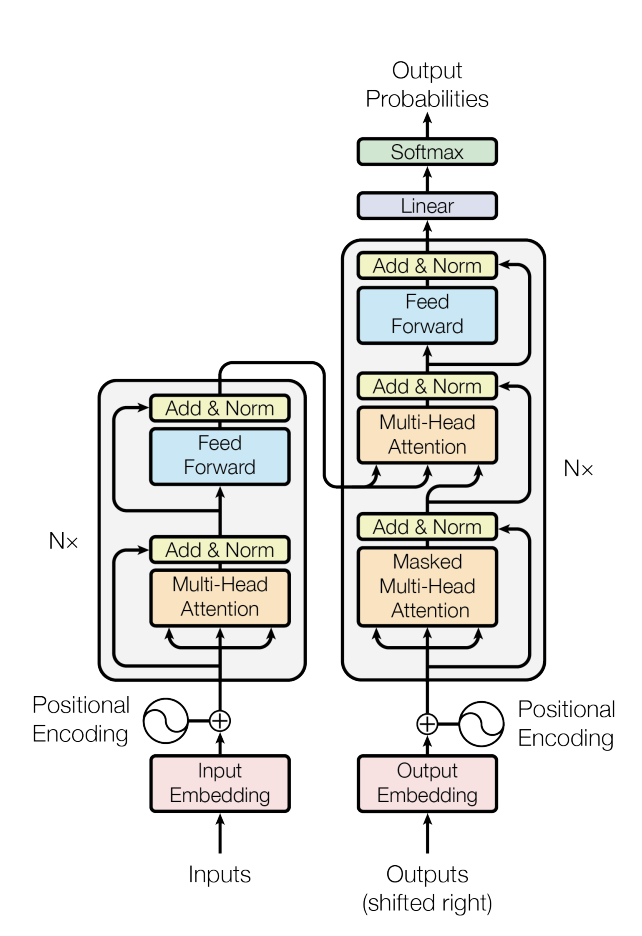
\includegraphics[width=0.5\textwidth, scale=0.8]{figures/2-sota/transformer.png}
    \caption[Transformer]{\textbf{Transformer} --- This illustration was taken from \cite{vaswani_attention_2017} and shows the general architecture of the base transformer. One can see that the constituents are pretty simple. These are simple word embeddings (which are not covered in this study), self-attention, and feedforward layers. The left side of the structure is called the encoder, while the right side is called the decoder.}
    \label{fig:transformer}
\end{figure}
\paragraph{Vector Quantised Variational AutoEncoder (VQ-VAE) (2018)} \label{sec:vq-vae}

The \acf{VQ-VAE}, introduced in 2018, model distinguishes itself from traditional \acp{VAE} in two main aspects: the encoder network outputs discrete codes instead of continuous ones, and the prior is learned rather than static. While continuous feature learning has been the focus of many previous works, this model, introduced by \cite{oord_neural_2018}, concentrates on discrete representations, a natural fit for complex reasoning, planning, and predictive learning.

The \ac{VQ-VAE} model combines the \ac{VAE} framework with discrete latent representations through a parameterization of the posterior distribution of (discrete) latents given an observation. Based on vector quantization, this model is simple to train, does not suffer from significant variance, and avoids the ``posterior collapse''. As illustrated in Fig~\ref{fig:vq-vae}, the \ac{VQ-VAE} architecture consists of an encoder, a discrete latent space, and a decoder.

\begin{figure*}[ht]
    \centering
    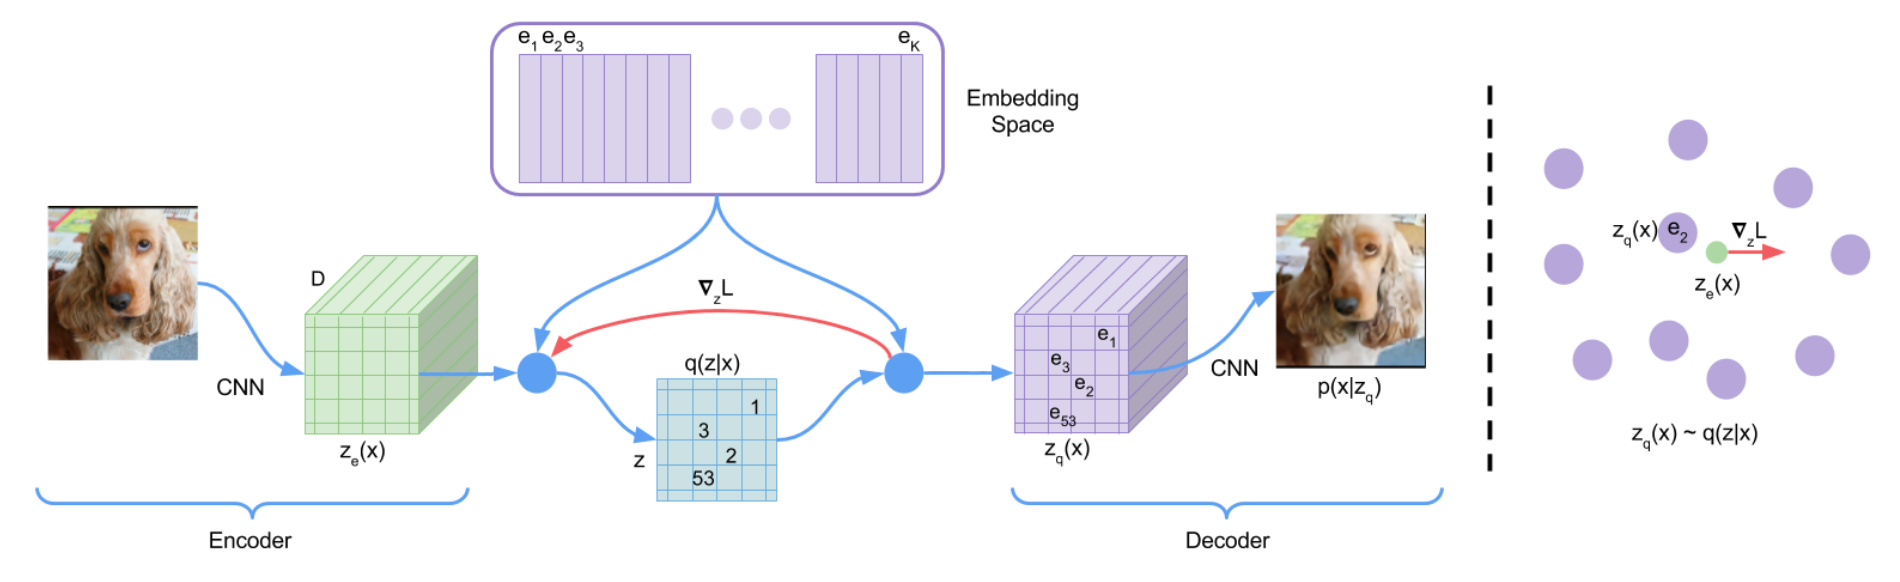
\includegraphics[width=\textwidth]{figures/2-sota/vq-vae.png}
    \caption[VQ-VAE]{\textbf{VQ-VAE} --- Taken from the original paper, this Figure presents two distinct illustrations. On the left side, a detailed diagram of the \ac{VQ-VAE} architecture is provided, showcasing the flow of information through the encoder, the discrete latent space, and the decoder. On the right side, a visualization of the embedding space is displayed, where the encoder output $z(X)$ is mapped to its nearest embedding point $e_2$. The red arrow represents the gradient $\nabla_z L$, influencing the encoder's output adjustment. This adjustment may result in a different configuration during the subsequent forward pass, highlighting the dynamic nature of the learning process within the \ac{VQ-VAE} model.}
    \label{fig:vq-vae}
\end{figure*}

The \ac{VQ-VAE} defines a latent embedding space $e \in R^{N \times D}$, where $N$ is the size of the discrete latent space (i.e., a $N$-way categorical), and $D$ is the dimensionality of each latent embedding vector $e_n$. There are $N$ embedding vectors $e_n \in R^D, n \in 1, 2, ..., N$. The model takes an input $X$, passed through an encoder producing output $z_e(X)$. The discrete latent variables $z$ are then calculated by the nearest neighbor look-up using the shared embedding space $e$. The input to the decoder is the corresponding embedding vector $e_n$. This forward computation pipeline is a regular autoencoder with a non-linearity that maps the latents to 1-of-N embedding vectors.

The posterior categorical distribution $q(z|X)$ probabilities are defined as one-hot (Eq. \ref{eq:vq-vae-posterior}):

\begin{equation} \label{eq:vq-vae-posterior}
  q(z = n|X) =
  \begin{cases}
    1 & \text{for } n = \text{argmin}_j ||z_e(X)-e_j||_2, \\
    0 & \text{otherwise}.
  \end{cases}
\end{equation}

where $z = e_n$ is the closest embedding vector to the encoder output $z_e(X)$. During forward computation, the nearest embedding $z_q(X)$ is passed to the decoder, and during the backward pass, the gradient $\nabla_z L$ is passed unaltered to the encoder. The overall loss function has three components to train different parts of the \ac{VQ-VAE}: the reconstruction loss, the \ac{VQ} objective, and the commitment loss. The total training objective becomes:

\setlength{\arraycolsep}{0.0em}
\begin{eqnarray}
\label{eq:vq-vae-loss}
\label{eq:reconstruction-loss}L&{}={}&\log p(X|z_q(X))\\
\label{eq:vq-objective}&&{+}\:||\text{sg}[z_e(X)] - e||_2^2\\
\label{eq:commitment-loss}&&{+}\:\beta||z_e(X) - \text{sg}[e]||_2^2
\end{eqnarray}
\setlength{\arraycolsep}{5pt}

This equation combines the three following terms:
\begin{enumerate}
	\item \textbf{Reconstruction loss} (Equation \ref{eq:reconstruction-loss}): This term represents the log probability of the input data $X$ given the latent variable  $z_q(X)$. It measures how well the model can reconstruct the input data using $z_q(X)$ as a representation. Maximizing this term would lead to a better reconstruction of the input data.
	\item \textbf{\Ac{VQ}} (Equation \ref{eq:vq-objective}): The second term measures the difference between the stop-gradient of the encoder output $z_e(X)$ and the embedding vector $e$. The stop-gradient operator, denoted as $\text{sg}$, acts as the identity during the forward pass but has zero partial derivatives during the backward pass. This term encourages the model to use the embeddings effectively by minimizing the distance between the encoder output and the closest embedding vector.
	\item \textbf{Commitment loss} (Equation \ref{eq:commitment-loss}): This term acts as a regularization term that measures the difference between the encoder output $z_e(X)$ and the stop-gradient of the embedding vector $e$. The  $\beta$ parameter controls the strength of this regularization. Minimizing this term would make $z_e(X)$  closer to the straight-through estimator of $e$.
\end{enumerate}

VQ-VAE has emerged as a vital component in generative artificial intelligence, spanning domains such as image~\cite{ramesh_zero-shot_2021} and sound generation~\cite{yang_diffsound_2022}.
\paragraph{Multi-Scale Vector Quantised Variational AutoEncoder (MS-VQ-VAE) (2019)} \label{sec:ms-vq-vae}

The \acf{MS-VQ-VAE} model is a generalization of the \ac{VQ-VAE} model (see Section \ref{sec:vq-vae}) that employs multiple discrete latent spaces with different scales and dimensions. Tjandra et al. proposed this model \cite{tjandra_vqvae_2019} to learn unsupervised hierarchical and discrete representations of complex data. The \ac{MS-VQ-VAE} architecture comprises an encoder, a multiscale discrete latent space, and a decoder.

The key difference between the \ac{MS-VQ-VAE} and the \ac{VQ-VAE} is that the former defines a collection of latent embedding spaces $e^s \in R^{K_s \times D_s}$, where $s$ denotes the scale index, $K_s$ denotes the cardinality of the discrete latent space at scale $s$, and $D_s$ denotes the dimensionality of each latent embedding vector $e^s_i$. There are $K_s$ embedding vectors $e^s_i \in R^{D_s}, i \in 1, 2, ..., K_s$. The model takes an input $x$, encoded into outputs $z_e^s(x)$ at different scales. The discrete latent variables $z^s$ are then obtained by the nearest neighbor look-up using the shared embedding space $e^s$. The decoder input is the corresponding embedding vector $e^s_k$. This forward computation pipeline resembles a regular \ac{AE} (see section \ref{sec:autoencoders}) with a non-linearity that maps the latents to 1-of-$K_s$ embedding vectors.

The posterior categorical distribution $q(z^s|x)$ probabilities are defined as one-hot (Eq. \ref{eq:ms-vq-vae-posterior}), analogous to Eq. \ref{eq:vq-vae-posterior} in section \ref{sec:vq-vae}, but with an additional scale index:

\begin{equation} \label{eq:ms-vq-vae-posterior}
 q(z^s = k|x) = \begin{cases}
 1 & \text{for } k = \text{argmin}_j ||z_e^s(x)-e^s_j||_2, \\
 0 & \text{otherwise}.
 \end{cases}
\end{equation}

The overall loss function consists of three components for each scale: the reconstruction loss, the VQ objective, and the commitment loss. The total training objective becomes (Eq. \ref{eq:ms-vq-vae-loss}), analogous to Eq. \ref{eq:vq-vae-loss} in section \ref{sec:vq-vae}, but with a summation over scales:

\begin{equation} \label{eq:ms-vq-vae-loss}
 L = \sum_{s=1}^{S} (\log p(x|z_q^s(x)) + ||\text{sg}[z_e^s(x)] - e^s||_2^2 + \beta||z_e^s(x) - \text{sg}[e^s]||_2^2)
\end{equation}

The benefit of using multiple codebooks and scales is that it enables the model to capture different levels of abstraction and granularity in audio signals. For instance, lower scales can encode phonetic information in speech, while higher scales can encode prosodic information. Furthermore, using multiple codebooks can enhance the diversity and expressiveness of the latent space by allowing more combinations of discrete codes.